\newpage
\section{Auswertung}
\label{sec:Auswertung}
Um aus den Messwerten des Reflektivitätsscans Schichtdicke, Dispersion
und Rauigkeit der Polysterolschicht, sowie Dispersion und Rauigkeit des Siliziumwafers
zu ermitteln, wird
% Untergrund von Messung mit Probe abziehen
zu Beginn der diffuse Scan von den Messwerten abgezogen, wie in Abbildung
\ref{fig:diffuse_Scan} zu sehen.

\begin{figure}
  \centering
  \includegraphics[width=0.7\textwidth]{build/plot_messung_untergrund}
  \caption{Reflektivitätsscan und diffuser Scan, sowie die Differenz von Reflektivitätsscan und diffusem Scan.}
  \label{fig:diffuse_Scan}
\end{figure}

Da erst ab einem ausreichend großen Einfallswinkel,
dem so definierten Geometriewinkel $\alpha_g$,
der gesamte Strahl auf die Oberfläche trifft,
werden die Messwerte mit $\alpha_i < \alpha_g$
mit einem Geometriefaktor $G$ korrigiert.
Dieser berücksichtigt den Intensitätsverlust, da
nicht der gesamte Strahl von der Probe reflektiert wird.
Der Geometriefaktor ergibt sich zu
\begin{align}
G&=\frac{D\sin\alpha_i}{d_0} &  &\text{für } \alpha_i<\alpha_g \label{eqn:GEO}\\
G&=1 & &\text{für } \alpha_i<\alpha_g \, .
\end{align}
Mit der Gesamtstrahlbreite $d_0$ und dem Durchmesser der Probenoberfläche $D$.
Ein beispielhafter Strahlverlauf für $\alpha_i<\alpha_g$ ist in Abbildung \ref{fig:geo}
dargestellt.
\begin{figure}
  \centering
  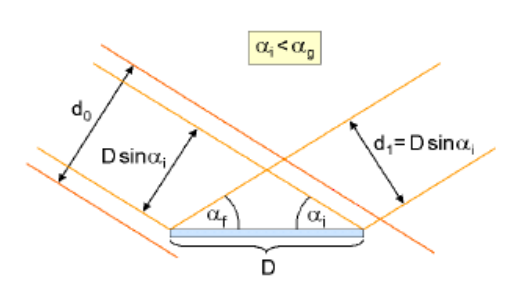
\includegraphics{bilder/geo_winkel.PNG}
  \caption{Strahlverlauf für $\alpha_i<\alpha_g$. \cite{sample}}
  \label{fig:geo}
\end{figure}

Der Strahldurchmesser $d_0$ und der Druchmesser der Probenoberfläche $D$ können in der Formel für den Geometriefaktor \eqref{eqn:GEO}
durch den Zusammenhang
\begin{align}
   \sin(\alpha_g) = \frac{d_0}{D}
\end{align}
mit dem Geometriewinkel $\alpha_g$ ersetzt werden, sodass der Geometriefaktor
\begin{align}
  G&=\frac{\sin\alpha_i}{\sin\alpha_g} &  &\text{für } \alpha_i<\alpha_g \label{eqn:GEO_neu}\\
  G&=1 & &\text{für } \alpha_i<\alpha_g
\end{align}
lautet.
Der Geometriewinkel ergibt sich aus den Messungen, die zu Justagezwecken vor der eigentlichen Messung durchgeführt werden.
Desweiteren wird die Intensität der einfallenden Strahlung $I_0$ benötigt, um die normierte Reflektivität
\begin{align}
  R=\frac{I_R}{I_0}
\end{align}
zu erhalten.
Aus den Messwerten des Detektorscans ergibt sich der in Abbildung \ref{fig:det_scan}
gezeigte Intensitätsverlauf in Abhängigkeit des Detektorwinkel $\Theta'$.

\begin{figure}
  \centering
  \includegraphics[width=0.7\textwidth]{build/plot_det_scan.pdf}
  \caption{Intensität in Abhängigkeit des Detektorwinkels $\Theta'$ während eines Detektorscans und Fit an die Intensitätsverteilung.}
  \label{fig:det_scan}
\end{figure}

Durch einen Fit der Form
\begin{align}
  I(\Theta) =  I_0 \exp\left(-\frac{(\Theta-\mu)^2}{\omega^2}\right) \text{\cite{wiki_strahl}}
\end{align}
an die Intensitätsverteilung, ergibt sich die Intensität
\begin{align}
  I_0 = \SI{9.12(3)e7}{}
  \label{eqn:I_0}
\end{align}
der einfallenden Strahlung.
% \begin{align}
% \mu&= & \omega&= \\
% \end{align}
% und dem Radius $R=\SI{0.5}{\meter}$?? folgt für den Strahldurchmesser
% \begin{align}
%   d_0=\SI{}{\meter}.
% \end{align}
% Zur Ermittelung der Probenoberfläche $D$ wird zunächst aus den Messwerten

Zur Ermittlung des Geometriewinkels  $\alpha_g$ werden die Messwerte
des Rockingscan mit $2\Theta = \SI{0}{\degree}$, die in der Abblidung \ref{fig:rock_scan_0}
dargestellt sind, verwendet.


\begin{figure}
  \centering
  \includegraphics[width=0.7\textwidth]{build/plot_rocking.pdf}
  \caption{Messwerte des Rockingscan mit $2\Theta = \SI{0}{\degree}$ und Fit.}
  \label{fig:rock_scan_0}
\end{figure}

Dafür wird eine Funktion der Form
\begin{align}
  f(x) = a \lvert x + b \rvert + c
\end{align}
an die Messwerte angepasst und es ergeben sich die Parameter
\begin{align}
  a&=-\num{150(2)e6}  &b&=\num{-0.220(2)}  &c&=\num{722(7)e5} \, .
\end{align}
Dabei entspricht der Parameter $b$ nur einer fehlenden Eichung in der Messung und
es wird für die Berechnung des Geometriewinkels $b=0$ gesetzt.
Der Geometriewinkel entspricht dem Winkel, ab dem der Strahl
vollständig auf die Probe trifft. Bei dem Rockingscan für $2\Theta=\SI{0}{\degree}$
entspricht der Geometriewinkel genau dem Winkel ab dem keine Intensität
mehr auf den Detektor fällt und somit genau dem Betrag der Nullstellen der an die Messwerte
angepassten Funktion.
Der bestimmte Geometriewinkel $\alpha_g$
lautet somit
\begin{align}
\alpha_g = \lvert \pm\frac{c}{a} \rvert = \SI{0.48(1)}{\degree}.
\end{align}
% Über den Zusammenhang
% \begin{align}
% D = d_0\sin(\alpha_g)
% \end{align}
% ergibt sich der Druchmesser
% der Probenoberfläche.
% \begin{align}
%   D=\Si{}{\meter}
% \end{align}


Die Messwerte $I_{\mathrm{mess}}$ mit $\alpha_i < \alpha_g $ werden mit dem Geometriefaktor $G$
in der Form
\begin{align}
  I_{\mathrm{korr}} = \frac{I_{\mathrm{mess}}}{G}
\end{align}
korrigiert. Die mit Hilfe des Geometriefaktors korrigierten Messwerte sind in der Abbildung \ref{fig:korr} dargestellt.
\begin{figure}
  \centering
  \includegraphics[width=0.7\textwidth]{build/Geometriefaktor.pdf}
  \caption{$I_{\mathrm{mess}}$ und normiertes $I_{\mathrm{korr}}$ in Abhängigkeit des Einfallswinkel $\alpha_i$.}
  \label{fig:korr}
\end{figure}

Ebenfalls in der Abbildung \ref{fig:korr}
sind die lokalen Minima im Refektivitätsscan markiert.
Über die Differenz der Einfallswinkel bei lokalen Minima lässt
sich der Schichtabstand $d$ nach Gleichung \eqref{eqn:schichtabstand}
bestimmen.
Dazu werden alle Differenzen
berechnet und über alle Werte gemittelt, wobei Einfallswinkel
über $\SI{2}{\degree}$ auf Grund von Signalstörungen vernachlässigt werden.
Es ergibt sich eine Differenz von $\Delta \alpha_i = \SI{0.053(3)}{\degree}$
und mit einer Wellenlänge von $\lambda=\SI{1.54}{\angstrom}$
ein Schichtabstand von
\begin{align}
d \approx \frac{\lambda}{2\Delta\alpha_i} = \SI{840(50)}{\angstrom}.
\end{align}
% Geometriewinkel aus daten von Justierung -> Korrekturfaktor G
% -> Daten korrigieren

Um aus den Daten der Reflektivitätsmessung Dispersion und Rauigkeit
der Probe, sowie des Substrats zu bestimmen, werden die Messwerte in der Form
Einfallswinkel $\alpha_i$ gegen die
normierte Reflektivität $R$ aufgetragen, wie in Abbildung \ref{fig:messung}
zusehen. Zusätzlich wird an die markierten Messwerte
eine Funktion gefittet, die
sich über den
modifizierten Parratt-Algorithmus für raue Grenzflächen ergibt und
aus der Versuchsanleitung \cite{sample} entnommen wird.

% Schichtdicke mit formel (9)
% Dispersionsprofil mit Parrot Alg. ( Lage des krit. Winkels anpassen)
% (modifizierte Fresnel Koeff.fuer Rauigkeit)
% restliche Parameter



\begin{figure}
 \centering
   \includegraphics[width=0.7\textwidth]{build/Programm.pdf}
   \caption{Normierte Reflektivität $R$ gegen den Einfallswinkel $\alpha_i$ aufgetragen und Fit an die markierten Messwerte.}
   \label{fig:messung}
\end{figure}

Aus den Parametern ergeben sich für Dispersion $n_i$, Rauigkeit $\sigma_i$ und Schichtdicke $d$ die Werte
\begin{align}
  n_{\mathrm{Schicht}}&= 1-\num{3.33(4)e-6}  & \sigma_{\mathrm{Schicht}}&= \num{17.9(5)e-10} \\
  n_{\mathrm{Substrat}}&=1-\num{7.33(4)e-6} & \sigma_{\mathrm{Substrat}}&= \num{4.6(1)e-10}\\ % ?? so richtig ?
  d& =\SI{815.4(9)}{\angstrom}
\end{align}
für die verwendete Probe.
Die Elektronendichte $\rho_i$ der zwei Materialien ergibt sich aus dem Zusammenhang \eqref{eqn:elektronendichte} zu
\begin{align}
\rho_i&=\frac{2\delta_i \pi}{\lambda^2 r_e} &\text{mit}&  &\delta_i = 1 - n_i.\\
\end{align}
Aus den berechneten Dispersionen ergeben sich die Elektronendichten
\begin{align}
\rho_{\mathrm{Schicht}}&=\SI{3.13(4)e29}{\per\cubic\meter}  & \rho_{\mathrm{Substrat}}&=\SI{6.89(4)e29}{\per\cubic\meter}
\end{align}
